% header
\documentclass[10pt,a4paper]{article}

\usepackage[utf8]{inputenc}
\usepackage{hyperref}
\usepackage{amssymb}
\usepackage{xcolor}
\usepackage{ngerman}
\usepackage{mathtools}
\selectlanguage{german} 
\usepackage[german,onelanguage]{algorithm2e} %for psuedo code
% the document
\begin{document}

% Ersetzt in den eckigen Klammern bitte die Übungsnummer.
\title{Abgabe - Übungsblatt [$8$]\\
\small{Einführung in die Computergraphik und Visualisierung}}
\author{ [Till Sebastian] \and [Felix Grefe] \and [Marius Rometsch]}
\date{\today}
\maketitle



\section*{Teilaufgabe 1}
\subsection*{b)}
Radiance (Strahldichte)
\\L$e_1(x,w_1)=\frac{d^2\phi e_1}{\cos(e_1)dAdw_1}[\frac{w}{srm^2}]$
\begin{itemize}
\item Leistung pro Einheitsraumwinkel je projizierter Einheitsfläche
\item Helligkeit(Photonendichte) eines Punktes in Richtung$w_1$
\end{itemize}
Irradiance (Bestrahlungsstärke)
\begin{itemize}
	\item Auftreffende Strahlungsleistung pro Fläche
	\\$E_e=\frac{d\phi e_2}{dA_2}=I_e\frac{\cos(\alpha_2)}{R^2}[\frac{w}{m^2}]$
\end{itemize}
\begin{itemize}
	\item Leistung pro Einheitsraumwinkel je projizierter Einheitsfläche
	\item Helligkeit(Photonendichte) eines Punktes in Richtung$w_1$
\end{itemize}
\subsection*{c)}
Raytracing
\\Aus VL:
\\ "...Raytracing vor allem für Szenen mit hohem spiegelnden und transparente Flächenanteil gut geeignet"

\begin{itemize}
\item[\textbf{Vorteil}] Beleuchtungsmodell muss nur in sichtbaren Objektpunkten berechnet werden
\item[\textbf{Nachteil}] Abtastung der Szene mit einem Strahl pro Pixel erzeugt i.d.R. Aliasing
\end{itemize}

\section*{Teilaufgabe 3}
\begin{figure}
	\centering 
	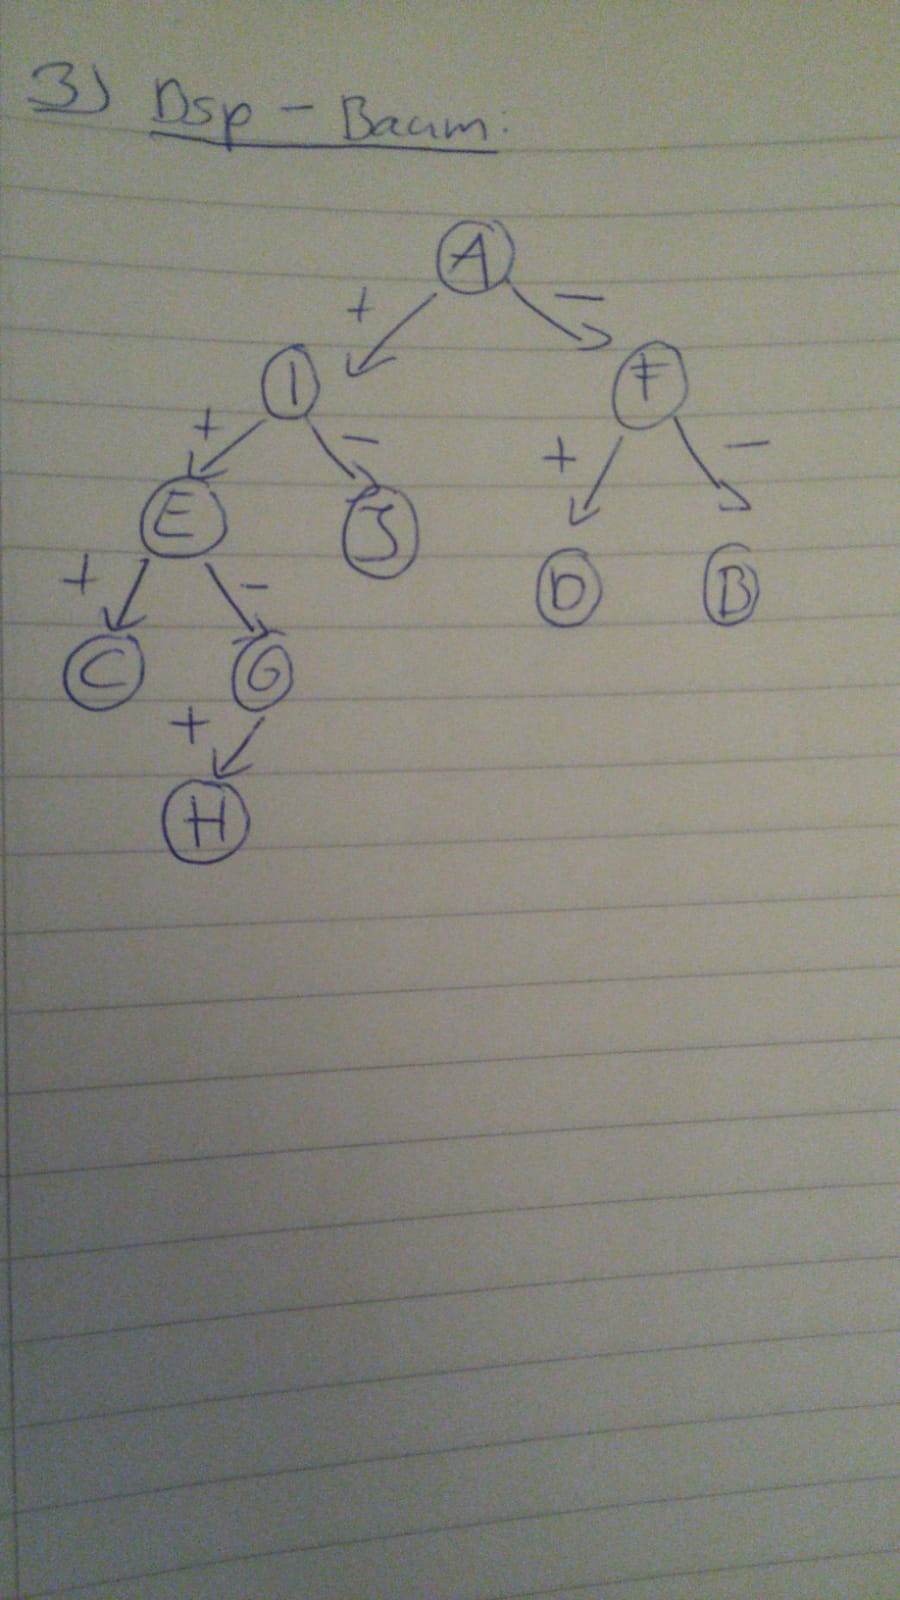
\includegraphics[width=1\textwidth]{A3.jpeg}
\end{figure}
\end{document}
